\documentclass{article}


\usepackage{graphics}
\usepackage{epsfig}
\title{Design Space ExploRation Tool}

\author{
Endre, Magyari\\
ISIS, Vanderbilt University\\
endre.magyari@vanderbilt.edu
}
\date{\today}

\begin{document}
\setcounter{figure}{1}
\maketitle

\vspace{3cm}
{\par\centering 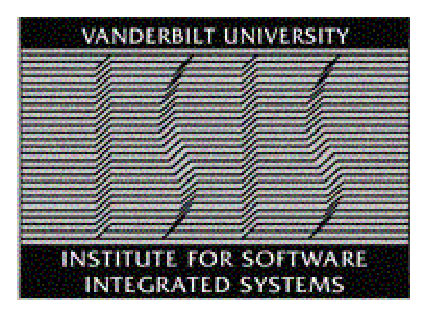
\includegraphics{isis.eps} \par}
\newpage
\section{Overview}
\section{Interface Models}
\begin{par}
The DESERT defines two APIs, one for submitting the data into DESERT,the Input Interface, and another one for dumping the output, the pruned Design Space, the Output or {\it Back} Interface. 
These interfaces and the API's are provided by the UDM Framework\cite{UDM}. The DESERT expects an input data network based on the input interface model, and outputs an output data network based on the output interface model. The input and the output data networks may persist on any of the supported UDM backends.
Both the input and the output interface are defined in form of UML class diagrams. 

\end{par}
\subsection{Input Interface Model}
{\par 
There are three different basic terms: {\tt Space}, {\tt Domain}, and {\tt Property}. }
\subsubsection{{\bf Spaces}}
\label{space}
\vspace{1cm}
\begin{center}
\epsfig{file=di_space.eps,height=2in,width=3in} 
{\par Input Interface Model: Hierarchial Space}
\end{center}
\vspace{1cm}

{\par By {\tt Space} we mean an {\tt AND-OR-LEAF} tree of elements. This, from the constraint satisfaction tool's point of view means that the {\tt OR} nodes are variables, and their possible values are their children. The type of the node it's controlled by it's {\tt decomposition} boolean attribute and the number of subelements(children) of a node in the following way:}
\begin{list}{}{}
\item{ If the number of children is $= 0$, then the type is {\tt LEAF}}
\item{ If the number of children is $> 0$ and {\tt decomposition}, then the type is {\tt AND}}
\item{ If the number of children is $> 0$ and not {\tt decomposition}, then the type is {\tt OR}}
\end{list}
{\par
  All the nodes may have {\tt Constraint}s (each {\tt constraint} has a {\tt context()} which is a node of any type), and the {\tt Constraint}s are contained in {\tt ConstraintSet}s. {\tt ConstraintSet}s are there just for the reason to provide a mechanism for grouping the {\tt Constraint}s in several categories, which are specific to application. Well, partially true: There is one special {\tt ConstraintSet}, the one with {\tt name} {\it "Implicit Constraints"}. The {\tt Constraint}s in this {\tt ConstraintSet} are automatically applied and not shown on the  DESERT user interface. The {\tt expression} attribute is the constraint expression, in an extended OCL language. This will be discussed in section \ref{const_l} in this document.}
{\par
{\tt ElementRelation}s are permitted between the {\tt Element}s to pass some extra information to the tool. These relations might be used when composing {\tt Properties}. Refer to section \ref{prop} for more information about element relations.
}
{\par {\tt DesertBase} is an abstract base class, each class in the input interface model is directly or indirectly inherited from this class. The value of the {\tt id} attribute should be unique for each UDM\cite{UDM} object passed to DESERT. The {\tt name} attribute is used in the {\tt Constraint} {\tt expression}, so, they should be unique as well at a certain level in the hierarchy. The {\tt externalID} attribute may carry extra information throughut DESERT about the object, which is application specific. The values if these attributes are presevered through DESERT, so this is how the application can identify and match the objects when reading them back from DESERT. 
}
{\par
  The {\tt DesertSystem} is just a container for everything in the input model. This is needed because of the nature of some of the UDM backends, which require everything to be contained in a ``RootObject''
}
\subsubsection{Properties}
\label{prop}
\vspace{1cm}
\begin{center}
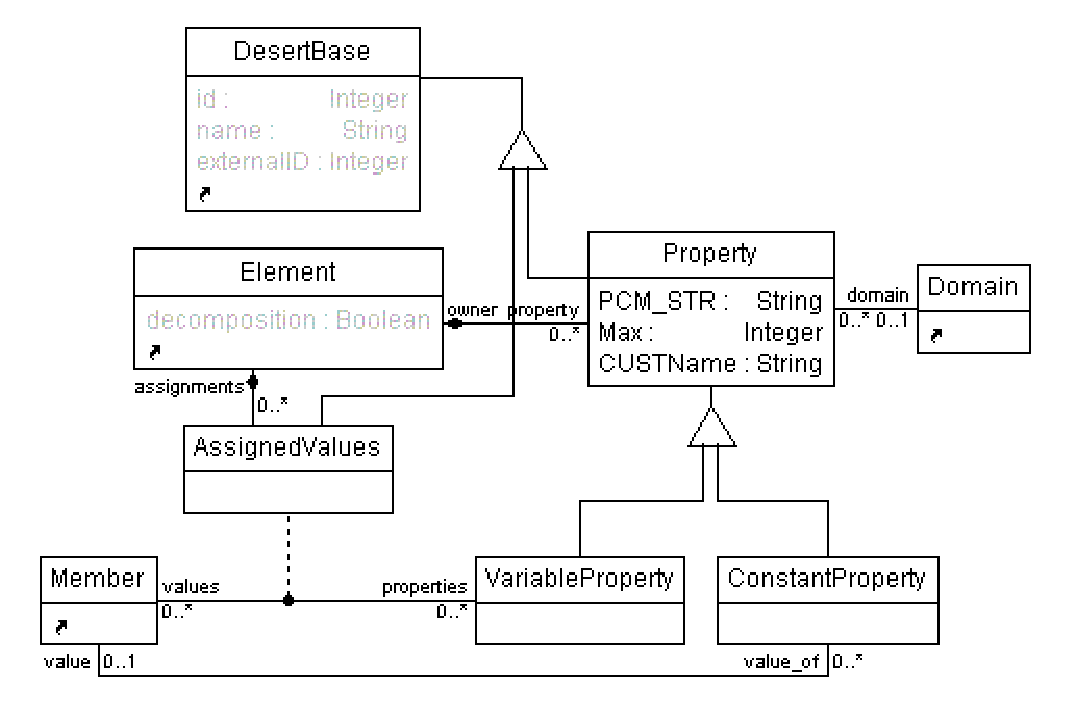
\epsfig{file=di_property.eps,height=2in,width=3in} \\
 Input Interface Model: Properties
\end{center}
\vspace{1cm}
{\par As mentioned above, leaf nodes can have {\tt Properties}. These {\tt Properties} then can be used to express {\tt Constraint}s. A {\tt Property} is owned by an {\tt Element} and always belongs to a {\tt Domain}. This is the set of {\tt Members} that can be assigned to {\tt Properties} as values. The {\tt Property} values can be composed in the {\bf AND-OR-LEAF} tree, if the {\tt Property} to be composed is defined for all the leaf nodes in the subtree rooted at the node at which the property should be evaluated.
The {\tt PCM\_STR} attribute specifies how a {\tt Property} should be composed, when the constraint engine needs to evaluate it at an {\tt AND} or an {\tt OR} compound node. The possible values for this attribute are:
}
{\par
\begin{list}{}{}
\item {{\tt PCM\_ADD} - specifies that the {\tt Property} is {\it additive} }
\item {{\tt PCM\_MUL} - specifies that the {\tt Property} is {\it multiplicative} }
\item {{\tt PCM\_AMED} - specifies that the {\tt Property} value of the compound node is equal to the  {\it arithmetic median} of the same {\tt Property} values of the children. }
\item {{\tt PCM\_GMED} - specifies that the {\tt Property} value of the compound node is equal to the {\it geomethric  median} of the same {\tt Property} values of the children. }
\item {{\tt PCM\_MIN} - specifies that the {\tt Property} value of the compound node is equal to the {\it minimum} of the same {\tt Property} values of the children. }
\item {{\tt PCM\_MAX} - specifies that the {\tt Property} value of the compound node is equal to the {\it maximum} of the same {\tt Property} values of the children. }
\item {{\tt PCM\_NONE} - specifies that the {\tt Property} is a {\it non-composable} {\tt Property}. Thus, forcing the constraint engine to evaluate it at a compound node by adding such a constraint at a compound node will generate an error}
\item {{\tt PCM\_CUST} - specifies that there will be a {\it custom function} linked against DESERT, which will compose this property whenever is needed.  The {\tt CUSTName} attribute will hold the name of the custom function.}
\end{list}
}
{\par There are two kinds of propeties. {\tt VariableProperty} and {\tt ConstantProperty}. }
{\par As one would easily guess, {\tt VariableProperties} will be the variables of the constraint engine, thus, they may be assigned to more than one {\tt Member}s. The assignments are done by the association class {\tt AssignedValues}, which are contained in {\tt Element}s. Each {\tt AssignedValues} object points to a {\tt Member} with it's {\tt values()} pointer and to a {\tt VariableProperty} with it's {\tt properties()} pointer. 
}
{\par {\tt ConstantProperties} are there to define {\tt Properties} which are constant for a leaf node. Even if this is not used directly by the constraint engine, it's still needed when one needs to evaluate a property at a compound node, which implies that a certain {\tt property} must be defined for each leaf node in the subtree.
}
{\par Again, anything is derived from the {\tt DesertBase} abstract base class. One should pay extra attention to the {\tt id} and {\tt externalID} attributes of the {\tt AssignedValues}, because DESERT will return with set of {\tt Configuration}s which will contain a set of valid {\tt Assignment}s. In most of the cases the application will need to match the {\tt Assignment} objects in the output data network with the {\tt AssignedValues} objects in the input data network. This will be possible, since the {\tt Assignemnt} object will preserve the {\tt id}s of the {\tt AssignedValues} objects. 
}
{\par The abstract base class {\tt Property} captures the common funtionalities in {\tt VariableProperties} and {\tt ConstantProperties}, that these are contained in the {\tt owner} {\tt Element}, they operate on a {\tt Domain}.}

\subsubsection{Domains}
\label{dom}
\vspace{1cm}
\begin{center}
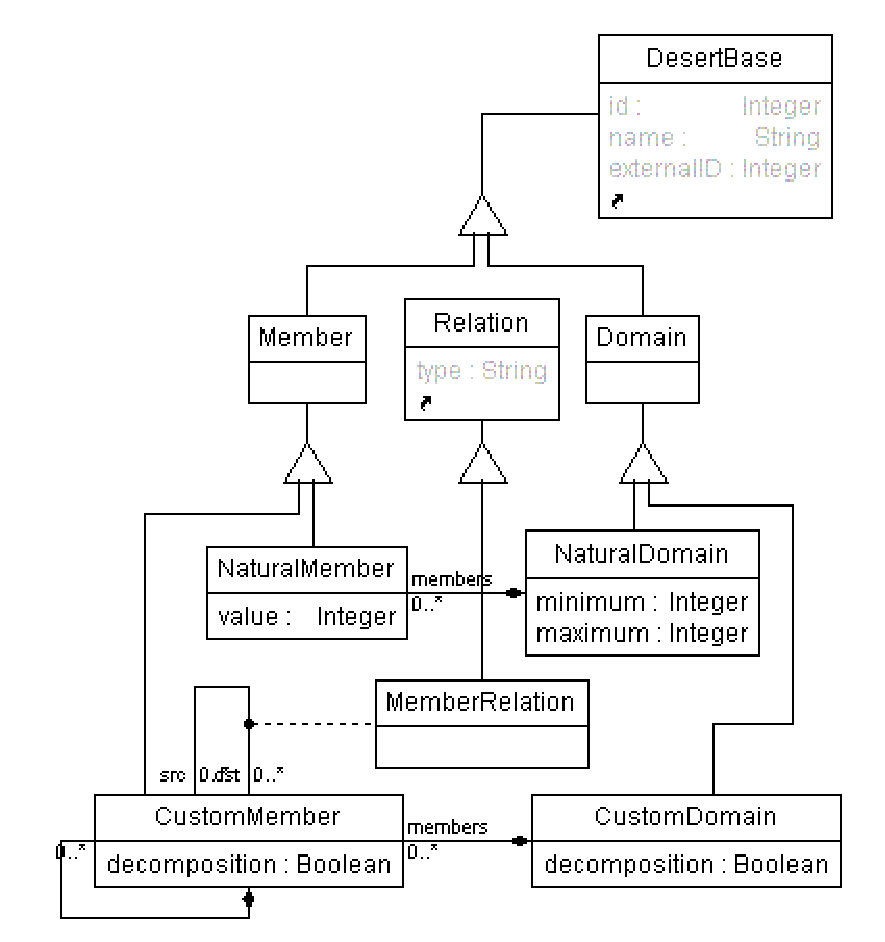
\epsfig{file=di_domain.eps,height=2in,width=3in} 
{\par
Input Interface Model: Domains}
\end{center}
\vspace{1cm}
{\par A {\tt Domain} is basically a set of values which {\tt Properties} may be assigned to. There are two kinds of {\tt Domain}s: {\tt CustomDomain}s and {\tt NaturalDomain}s.
}


{\par The {\tt CustomDomain} is  again an {\tt AND-OR-LEAF} tree and it has the same syntax as {\tt Space}. However, the {\tt decomposition} attribute is currently not used in the DESERT. The nodes of this tree are the {\tt CustomMember}s, which act exactly the same way as {\tt Elements} in the {\tt Space}. {\tt MemberRelation}s are there for the same reason {\tt ElementRelation}s are there. One could use this information in a custom function when composing {\tt Properties}.
}


{\par The {\tt NaturalDomain} is a set of natural numbers, which is defined by it's attributes {\tt minimum} and {\tt maximum}. However, if one wants to actually assign a value from a natural domain, then one would need to create a {\tt NaturalMember} with that value in the natural domain. 
}
{\par The abstract base class {\tt Member} captures the common functionality of {\tt CustomMember}s and {\tt NaturalMember}s. {\tt Member}s can be assigned as values to {\tt Properties}.
}

{\par The abstract base class {\tt Domain} captures the common functionality of {\tt CustomDomain}s and {\tt NaturalDomain}s that there are {\tt Properties} assigned to them.
}



\subsection{Output Interface Model}
\label{do}
\vspace{1cm}
\begin{center}
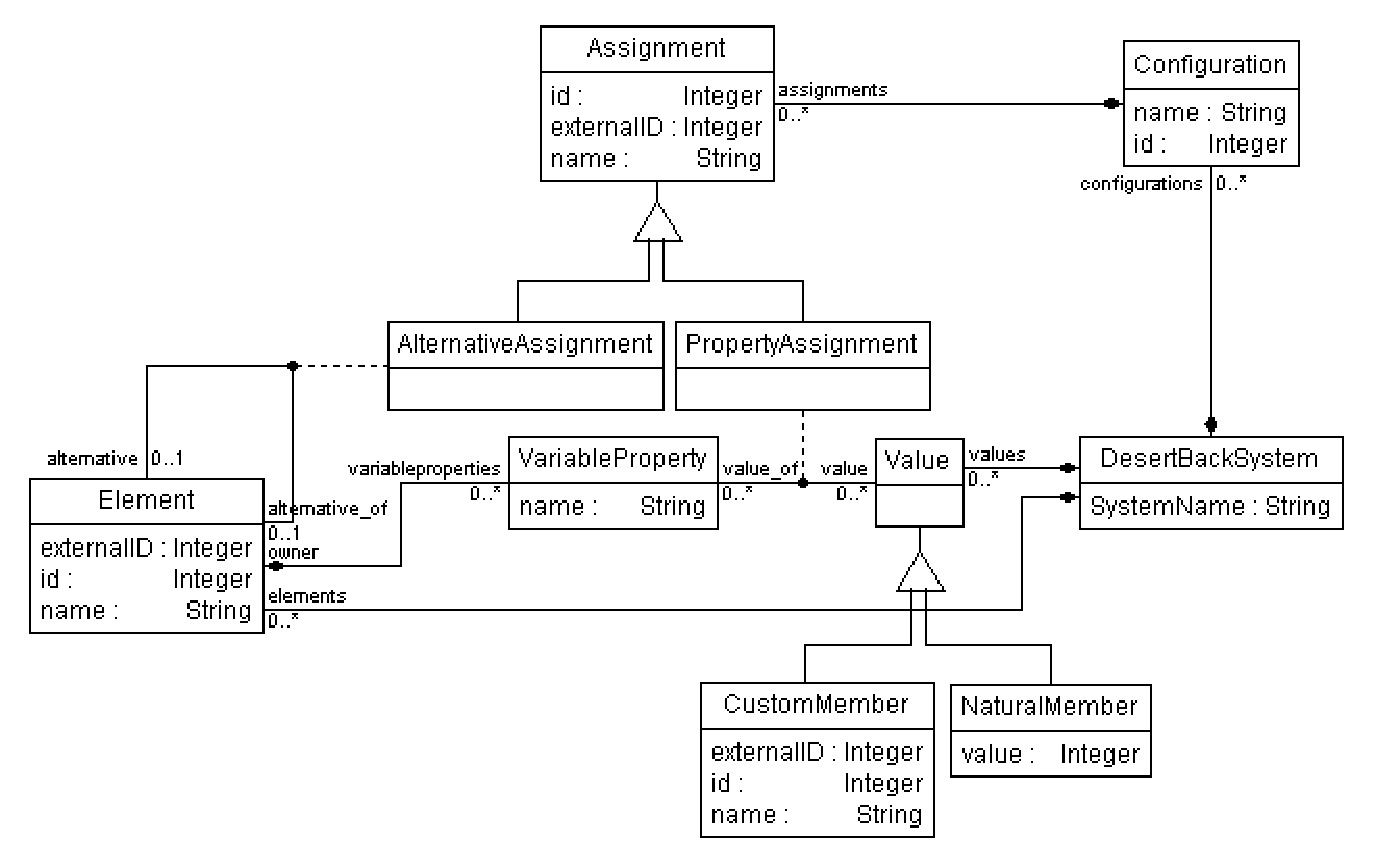
\epsfig{file=do.eps,height=3in,width=4in} 
{\par
 Output Interface Model}
\end{center}
\vspace{1cm}
{\par
The above class diagram was designed based on the idea that DESERT outputs valid {\tt Configuration}s which satisfy the applied {\tt Constraint}s. Each {\tt Configuration} will have exactly one  {\tt NaturalMember} or {\tt CustomMember} assigned to each {\tt VariableProperty}, and exactly one node(:={\tt Element}) for each compound node of type {\bf OR} in {\tt Space}.
}
{\par
The {\tt DesertBackSystem} is a class which contains everything. This will be the type of the root object of the output data network.  {\tt DesertBackSystem} contains {\tt values()}, {\tt elements()} and {\tt  configurations()} which are objects of type {\tt Value}, {\tt Element}, and {\tt Configuration}, respectivelly.  Further, the {\tt Element}s contain {\tt VariableProperties}. {\tt Element}s and {\tt VariableProperties} have exactly the same semantics as in the input interface model[\ref{space}]. 
A {\tt Configuration} object identifies a particular configuration in the design space. The valid {\tt Configuration}s are numbered, beginning from 1, and these are the values of their {\tt id} attribute. The {\tt name} {\tt Property} values will set to {\it ``Conf. no. x''} where {\it x} is the number of the {\tt Configuration}. A {\tt Configuration} contains {\tt Assignments}, which can be of two kinds: {\tt PropertyAssignment} and {\tt AlternativeAssignment}.  {\tt AlternativeAssignment}s assign a compound {\tt OR} node ({\tt alternative\_of()}) to a child node ({\tt alternative()}). {\tt PropertyAssignment}s assign a {\tt Value} to a {\tt VariableProperty}. However, if there are multiple {\tt AssignedValue}  objects in the input data network assigning the same {\tt Member} to the same {\tt VariableProperty}, for each such {\tt AssignedValue} object there will be a {\tt PropertyAssignment} object in the output data network. The {\tt Value} objects, and it's derivates, {\tt CustomMember} and {\tt NaturalMembers}  correspond to the {\tt Member}, {\tt CustomMember} and {\tt NaturalMember}  objects, respectivelly,  defined in the input interface model[\ref{dom}].
}
{\par The values of the {\tt id, externalID} attributes of the objects in the output data network are equal to the values of  the {\tt id} and {\tt externalID} attributes of the coresponding objects defined in the input interface model[\ref{dom}].
}

\section{The Constraint Language}
\label{const_l}
The constraint language in DESERT is an extended OCL. 
\subsection{Command Reference for the extensions:}
{\bf Global functions}\\
{\it project()} - returns the DESERT project\\
{\bf Project functions}\\
{\it name()} - returns the {\tt Space} or {\tt CustomDomain} named {\it ``name''}\\
{\bf {\tt Space} and {\tt CustomDomain} functions:}\\
{\it children()}- returns the collection of children(not recursive) nodes of a {\tt Space} or a {\tt CustomDomain}\\
{\it children(``name'')} - returns the node named {\it ``name''} from the children of a {\tt Space} or a {\tt CustomDomain}\\
{\bf {\tt CustomMember} and {\tt Element} (node) functions:}\\
{\it children()}- returns the collection of children(not recursive) nodes of a node\\
{\it children(``name'')} - returns the node named {\it ``name''} from the children of a node\\
{\bf {\tt Element} functions:}\\
{\it implementedBy()} - for an {\tt OR} type node returns the selected alternative(:=the value) from the children\\
{\it name()} - returns the value of the {\tt Property} named {\it ``name''} for the node. If this {\tt Property} operates on a {\tt CustomDomain}, it will return a {\tt CustomMember}, if it operates on a {\tt NaturalDomain}, it will return with an arithmetic value. If the context is a leaf node, it will directly read it's {\tt Property} value, if it's not, it will return a composed value. Note that non-composable {\tt Properties} can not be evaluated at compound nodes.\\


\section{Case study: Desert in MILAN}
\begin{thebibliography}{99}
 \bibitem{UDM} \'Arp\'ad, B., Endre, M. {\it The UDM Framework}, March 11, 2002.
 \end{thebibliography}
\end{document}
